\chapter{Architecture in Distributed Applications}
\label{ch:architecture}

\textit{The previous chapter presented the BCA system and the many challenges the chosen architecture introduced. This chapter will follow up on the case description and explain the evolution of software architecture, elaborating on three fundamentally different ways of structuring software projects.}

Architecture has very different meanings in respect to software development, this chapter will try and capture three of the more prominent architecture patterns distributed systems have been designed after the last 40 years: Monolithic, Service Oriented Architecture (SOA) and the newest addition Microservices. Each new iteration of dominant architecture pattern has been born from the previous, incorporating valuable lessons, trying to avoid pitfalls with earlier architectures. A recurring theme is increasing the granularity with which the system is partitioned, moving from Mono to Micro.

The Oxford dictionary uses \textit{Conceptual Structure} and \textit{Logical Organization} in their definition of architecture in software development, giving a good idea of what architecture can introduce in software development:
 
\defi{Architecture (Oxford)}{The conceptual structure and logical organization of a computer or computer-based system}{\url{https://en.oxforddictionaries.com/definition/architecture}} 
 
This of course is a very broad dictionary definition of the term, at the same time, this shows us some fundamental aspects of architecture. Architecture is indeed different sets of concepts, revolving around how we structure our software logically. Martin Fowler introduces his book \textit{Patterns of Enterprise Application Architectures} with the following statement about architecture \cite[p.~1]{fowler2002patterns}: \textit{"'Architecture' is a term that lots of people try to define, with little agreement. There are two common elements: One is the highest-level breakdown of a system into its parts; the other, decisions that are hard to change."}. According to Fowler, a architecture should break down a system into several parts, at the same time a architecture should take 'hard to change' decisions into account. 

Michael Nygaard states the following about a specific architectural decision (in this case about decoupling middleware) \cite[p.~116]{nygard2007release}: \textit{Decoupling Middleware is an architecture decision. It Ripples into every part of the system. This is one of those nearly irreversible decisions that should be made early rather than late}

Many factors have influenced software architecture through time. Available languages, frameworks and tools has drastically changed how software is developed today. Competition has also had it's influence by setting new requirements to the speed of development, having short and agile release cycles has never been more important \cite[t.~6:55]{george2016it}. Creating an architecture that supports these factors, makes it possible to utilize them, which in turn improves all parts of software development.

As it is with many things, it is never a silver bullet, decisions about the fundamental architecture of a system should be grounded in great understanding of what a specific architectural pattern incurs, and what the specific architecture helps mitigate. Vernon Vaughn states the following in the introduction for his Architecture chapter in his book \textit{Implementing Domain-Driven Design} \cite[p.~113]{vernon2013implementing}: \textit{“The following architectural styles and patterns are not a grab bag of cool tools we should apply everywhere possible. Instead, use them only where applicable, where they mitigate a specific risk that would otherwise increase the potential for project or system failure"}.

\section{Domain Driven Design}
\label{sec:DDD}
The DDD term was coined by Eric Evans in his book of the same name from 2004 \cite[preface]{evans2004domain}. Evans works with the notion that any complex domain should be partitioned into smaller subdomains, making it possible to comprehend the different subdomains and how a good solution can be created in that part of the domain. Models express a deep understanding of a particular subdomain, defining a model makes it possible to talk about the domain internal in a development team and externally with other development teams or customers. The model is a product of careful analysis of the domain, and should be reflected in the implementation, so that the analysis of the domain is visible in the code. This makes it possible to understand the implementation, and helps when maintaining and updating the application \cite[p.~2]{evans2004domain}.

Evans deems it very important that a model is kept simple, emphasizing the need for having several subdomains with their own model. Having a single model for a large system is not feasible or cost-effective \cite[p.~331]{evans2004domain}. By introducing what he calls \textit{Bounded contexts}, a models applicability is limited. A model is created in relation to a certain context, and this context will vary between each subdomain, concepts will likely occur in several subdomains, but might have very different meanings. Sharing a model across bounded contexts might hide the fact that there is a discrepancy in how the model is utilized, which can cause buggy and unreliable software, that is hard to understand. By limiting usage of a model, by explicitly defining bounded contexts, teams have a clear understanding of what is consistent across context and how it relates to their context \cite[p.~331]{evans2004domain}. Figure \ref{fig:architecture_bounded_context} shows a limited part of the domain for the earlier described BAC system, with two bounded contexts. The two contexts have a external and internal view of their User and Functionality package models, clearly showing how the two distinguish. The two contexts have dependencies across boundaries, indicating integration points.

\begin{figure}[!htb]
  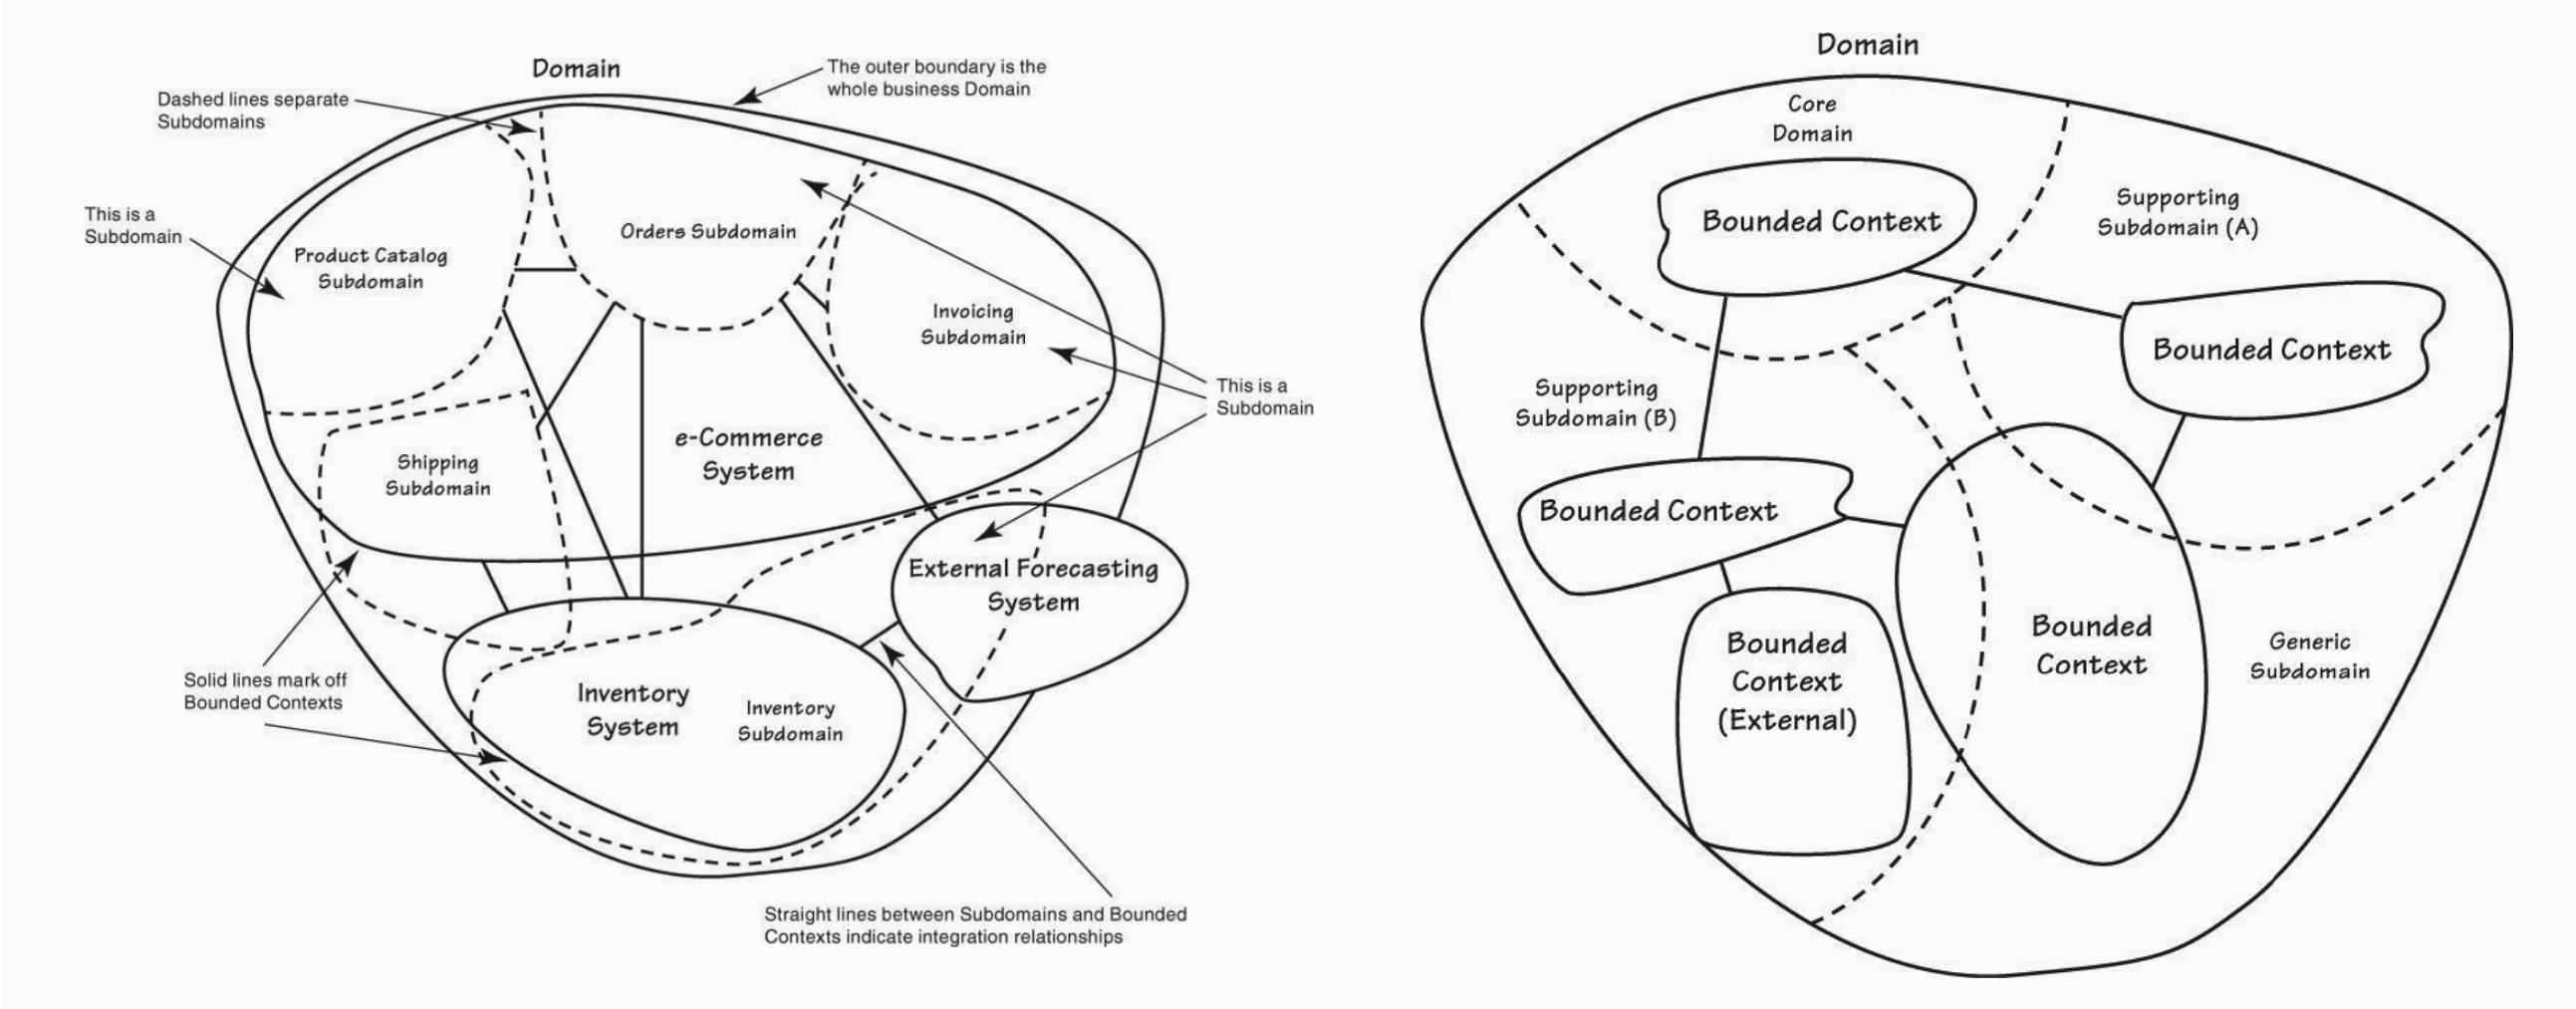
\includegraphics[width=\textwidth]{architecture_bounded_context}  
  \caption{An example of bounded context}
  \label{fig:architecture_bounded_context}
\end{figure}

According to Principal Consultant James Lewis and Chief Scientist Martin Fowler at ThoughtWorks, DDD is very useful when designing distributed applications \cite{fowler2014microservices}:

\tquote{DDD divides a complex domain up into multiple bounded contexts and maps out the relationships between them. This process is useful for both monolithic and microservice architectures, but there is a natural correlation between service and context boundaries that helps clarify, and as we describe in the section on business capabilities, reinforce the separations}{Lewis and Fowler}{2014}

According to Lewis and Fowler, DDD is usable, generally when designing applications, mentioning how separation between bounded contexts is more explicit when using microservices, highlighting one of the key features of the architecture, reducing the risk of sharing model across bounded contexts because of the explicit boundaries between services. The microservice architecture will be explored in further detail in section \ref{sec:microservices}.

\section{Monolithic}
The word monolith describes a application that exists as an single unit. By having the entire application as a single entity, the source code can be developed and managed together, giving multiple short term advantages \cite[p.~68]{long2017cloud}. Functionality can easily be added on top of a existing code base, giving the many advantages of low level programming language constructs. Communication can be done internally, between processes, not relying on non-deterministic network communication channels. 
According to Lewis and Fowler\cite{fowler2014microservices} enterprise web applications are often created as a monolith, consisting of three main parts: a client-side user interfaces, a shared common database management systems and a monolith server-side applications. The server-side application is a large and complex application, packed into a single executable. The application binds interface and database together, executing domain logic based on user input, retrieving and updating data as needed.
As the application grows in size, immediate advantages fade. The code base reaches a size where small changes in one part of the application might incur unforeseen changes in other parts. Centralizing the application decreases risk of failure, but at the same time forces development teams to coordinate changes, making sure breaking changes are not introduced \cite[p.~68]{long2017cloud}. 
According to Eric Evans having a single and unified model for a large system is not feasible nor cost-effective, and have several potential pitfalls if legacy code is updated by several teams simultaneously. Coordination might halt the project completely. The unified model may not be sufficient for some parts of the application, forcing functionality in elsewhere. Having a unified model leads to a very complex model that tries to encapsulate all aspects of the particular domain, making it difficult to use and therefore defeating the purpose \cite[p.~331]{evans2004domain}.

\subsection{Netflix -- the Transition away from the Monolith}
According to Meshenberg \cite{meshenberg2016microservices} Netflix previously had a monolithic implementation of their website. Each team would contribute a JAR file, that would be gathered into a single WAR file, that was deployed on a internal infrastructure. According to Meshenberg, this kind of architecture is very unreliable, mentioning that any issue introduced in either of the JAR files would be propagated onto all copies of the single service site executable. More importantly, the old architecture had a single relational database management system (RDBMS), creating a single point of failure\cite{meshenberg2016microservices}. Netflix experienced a outage, where their central RDBMS failed and caused wide system failure, resulting in four days with downtime. According to Meshenberg this event started the Netflix transition from a monolith to a microservice architecture.


\begin{figure}[!htb]
\begin{center} 
  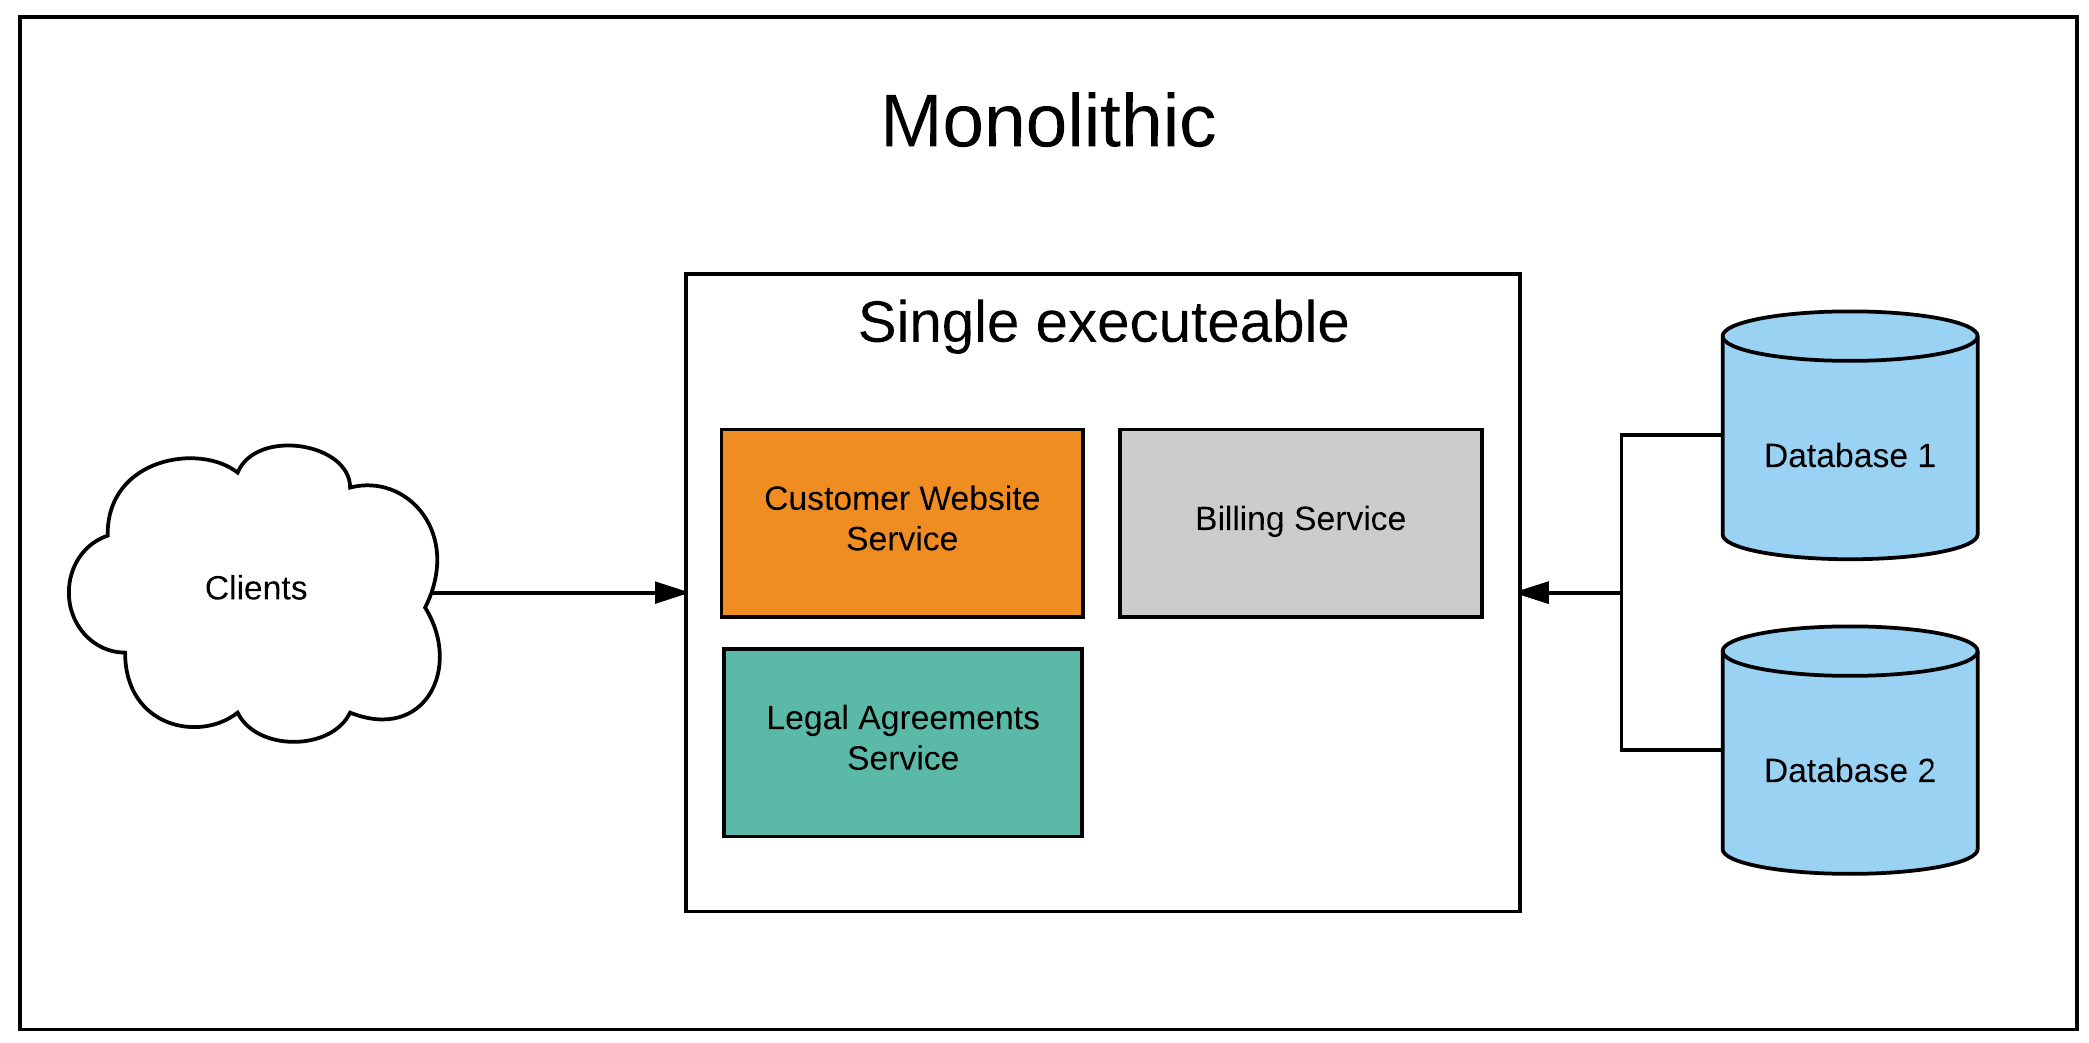
\includegraphics[scale=0.15]{architecture_monolithic_definition}  
  \caption{A monolithic setup, with a single executable containing all code. The executable is often put behind a load balancer, so it can be replicated, serving more load, this is how Meshenberg depicts the previous monolithic Netflix architecture}
  \label{fig:architecture_monolithic_definition}
  \end{center} 
\end{figure}

\section{Service-Oriented Architecture}
The SOA term has developed many different meanings \cite{microsoft2017chapter, george2016it, murer2015fifteen, sosinsky2010cloud, fowler2014microservicesoamonolith} since it was popuralised in the early to mid 2000 \cite[t.16:00]{george2016it}. This section will try and pin down which commonalities the many SOA definitions have.

Stephan Murer and Claus Hagen present Credit Suisse's (a financial service company well known for their early adoption of SOA) successful transformation of their tightly integrated monolith architecture to open SOA services  \cite{murer2015fifteen}: \textit{"The Service-Oriented Architecture (SOA) style has become a mainstream pattern for the design of large distributed systems over the past decade. The main idea behind SOA is to design a system as a network of interacting services. Each service provides clearly specified functionality over a well-defined interface"}. Credit Suisse successfully implemented a SOA, with focus on finding the right balance between quality control, strictness and agility when reviewing newly implemented services.

Microsoft has their own deifinition of SOA available on their MSDN website, stating that the only commonalities in the ambigous SOA term is the infrastructure capabilities: \textit{"A loosely‐coupled architecture designed to meet the business needs of the organization"} \cite{microsoft2017chapter}, emphasizing that SOA does not dictate specific technology but mere a pattern of design, that should push the system architecture towards a system that fulfils organisational needs.

Barrie Sosinsky also focuses on SOA as a definition for a standard of communication in a distributed component based system: \textit{"Service Oriented Architecture (SOA) describes a standard method for requesting services from distributed components and managing the results"} \cite{sosinsky2010cloud}. Sosinsky takes a more opinionated view of how SOA should be implemented mentioning several commonly used technologies.

More notably is Martin Fowler's talk about microservices at GOTO Berlin 2014 stating the following about the service oriented architecture the enterprise service bus (ESB) and how it is often a crucial part of the architecture:
\textit{When a lot of people talk about service oriented architecture they talk about the idea of 'let's get some powerful piece of middleware' that will automatically do all sorts of stuff it will route message it will apply business rules it does all sorts of things, this of course is the ESB the enterprise service bus or as it is more correctly know, the egregious spaghetti box} \cite[t.8.15]{fowler2014microservicesoamonolith}.

The common denominator in these many definitions of SOA is a system consisting of encapsulated and well defined components, communicating through a powerful service bus. The ESB is used by connected services to communicate, messages are send to the bus, with attached metadata containing information about the tasks needing to be solved for a given client application. SOA often incorporates a high amount of middleware implemented as part of the ESB between connected components. The middleware can contain business logic, taking several forms, from very industry-specific to more general purpose applications. SOA often utilizes Simple Object Access Protocol (SOAP) for message-passing, passing Extensible Markup Language (XML) documents between services \cite[p.~272]{sosinsky2010cloud}. Figure \ref{fig:architecture_soa} shows a SOA archiecture, every service in the system is interconnected through the ESB, making it a central part of SOA.

\begin{figure}[!htb]
\begin{center} 
  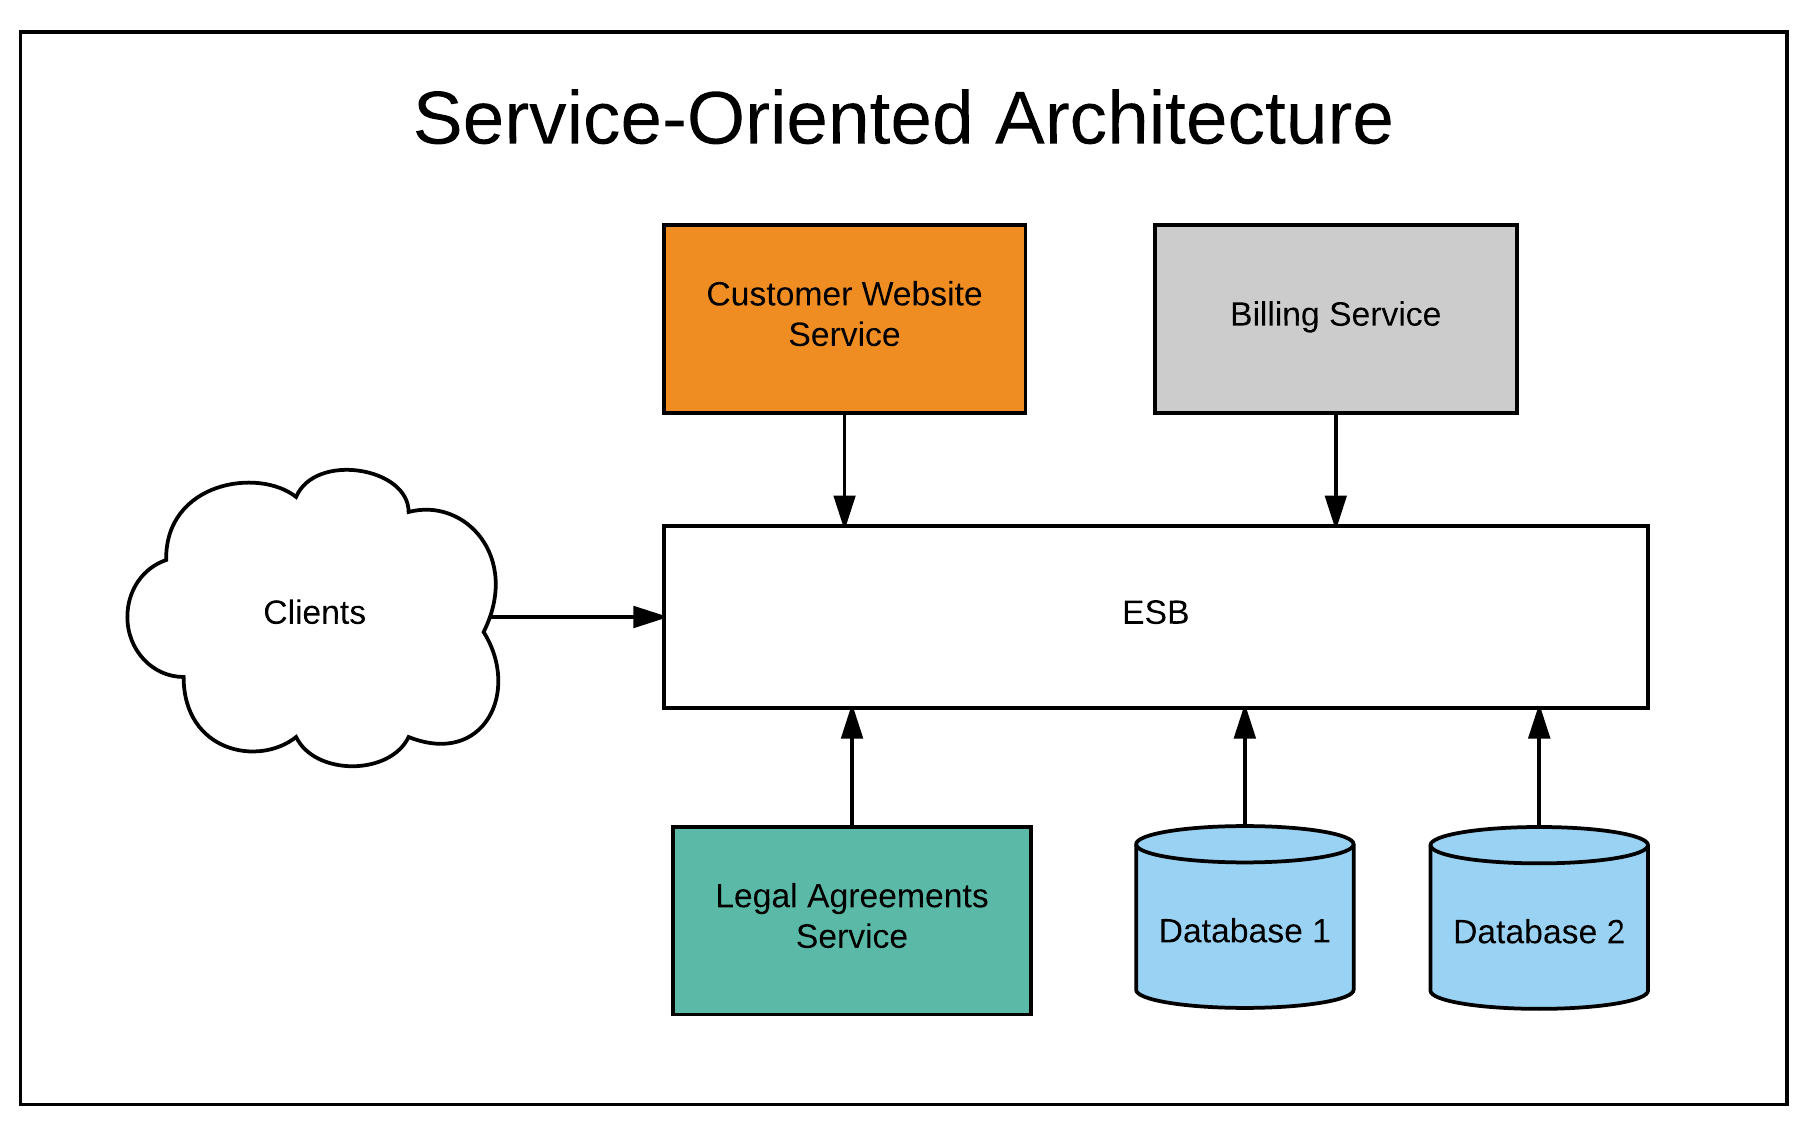
\includegraphics[scale=0.15]{architecture_soa}  
  \caption{A SOA architecture, incorporating the ESB as a central communication channel}
  \label{fig:architecture_soa}
  \end{center}
\end{figure}

SOA has many different meanings, which according to Fowler is also one of the main problems with SOA as a term \cite[t.13:12]{fowler2014microservicesoamonolith}. According to Fowler for some SOA has a very bad connotation, implying strict organisational regulation, determining how the system should be organised: Committees that lay down standards for how services connect to each other: \textit{"in my view the SOA term is too broad I mean, it means so many different things it is practically meaningless.. "}\cite[t.14:00]{fowler2014microservicesoamonolith}. Fowler criticizes SOA for relying heavily on ESB, containing advanced middleware products managing communication between services.

\section{Microservices}
\label{sec:microservices}
Microservice architecture gives an application composed of many small intercommunicating services. Each individual service has well defined and limited functionality and a well defined interface for external communication. Services communicate with each other through their interfaces and together they achieve a overarching business goal\cite[p.~2]{newman2015microservices}. A microservice architecture is shown on Figure \ref{fig:architecture_microservice_definition}, showing three individual services, each serving different purposes. The microservices are independently deployable and scaleable, if one service is more utilized than others, the specific container can easily be replicated, satisfying demand. \\

Having small and independently deployable services makes it possible to update services as teams identify problems or add new features. This supports agile software development, giving the flexibility and agility that the monolithic implementation lacks. By having small services, creating a modular, easy readable and understandable architecture is easier. Each service can be developed, tested and deployed independently, by the team creating it, minimizing the need for coordination between teams\cite{kniberg2014spotify}.

\begin{figure}[!htb]
\begin{center}
  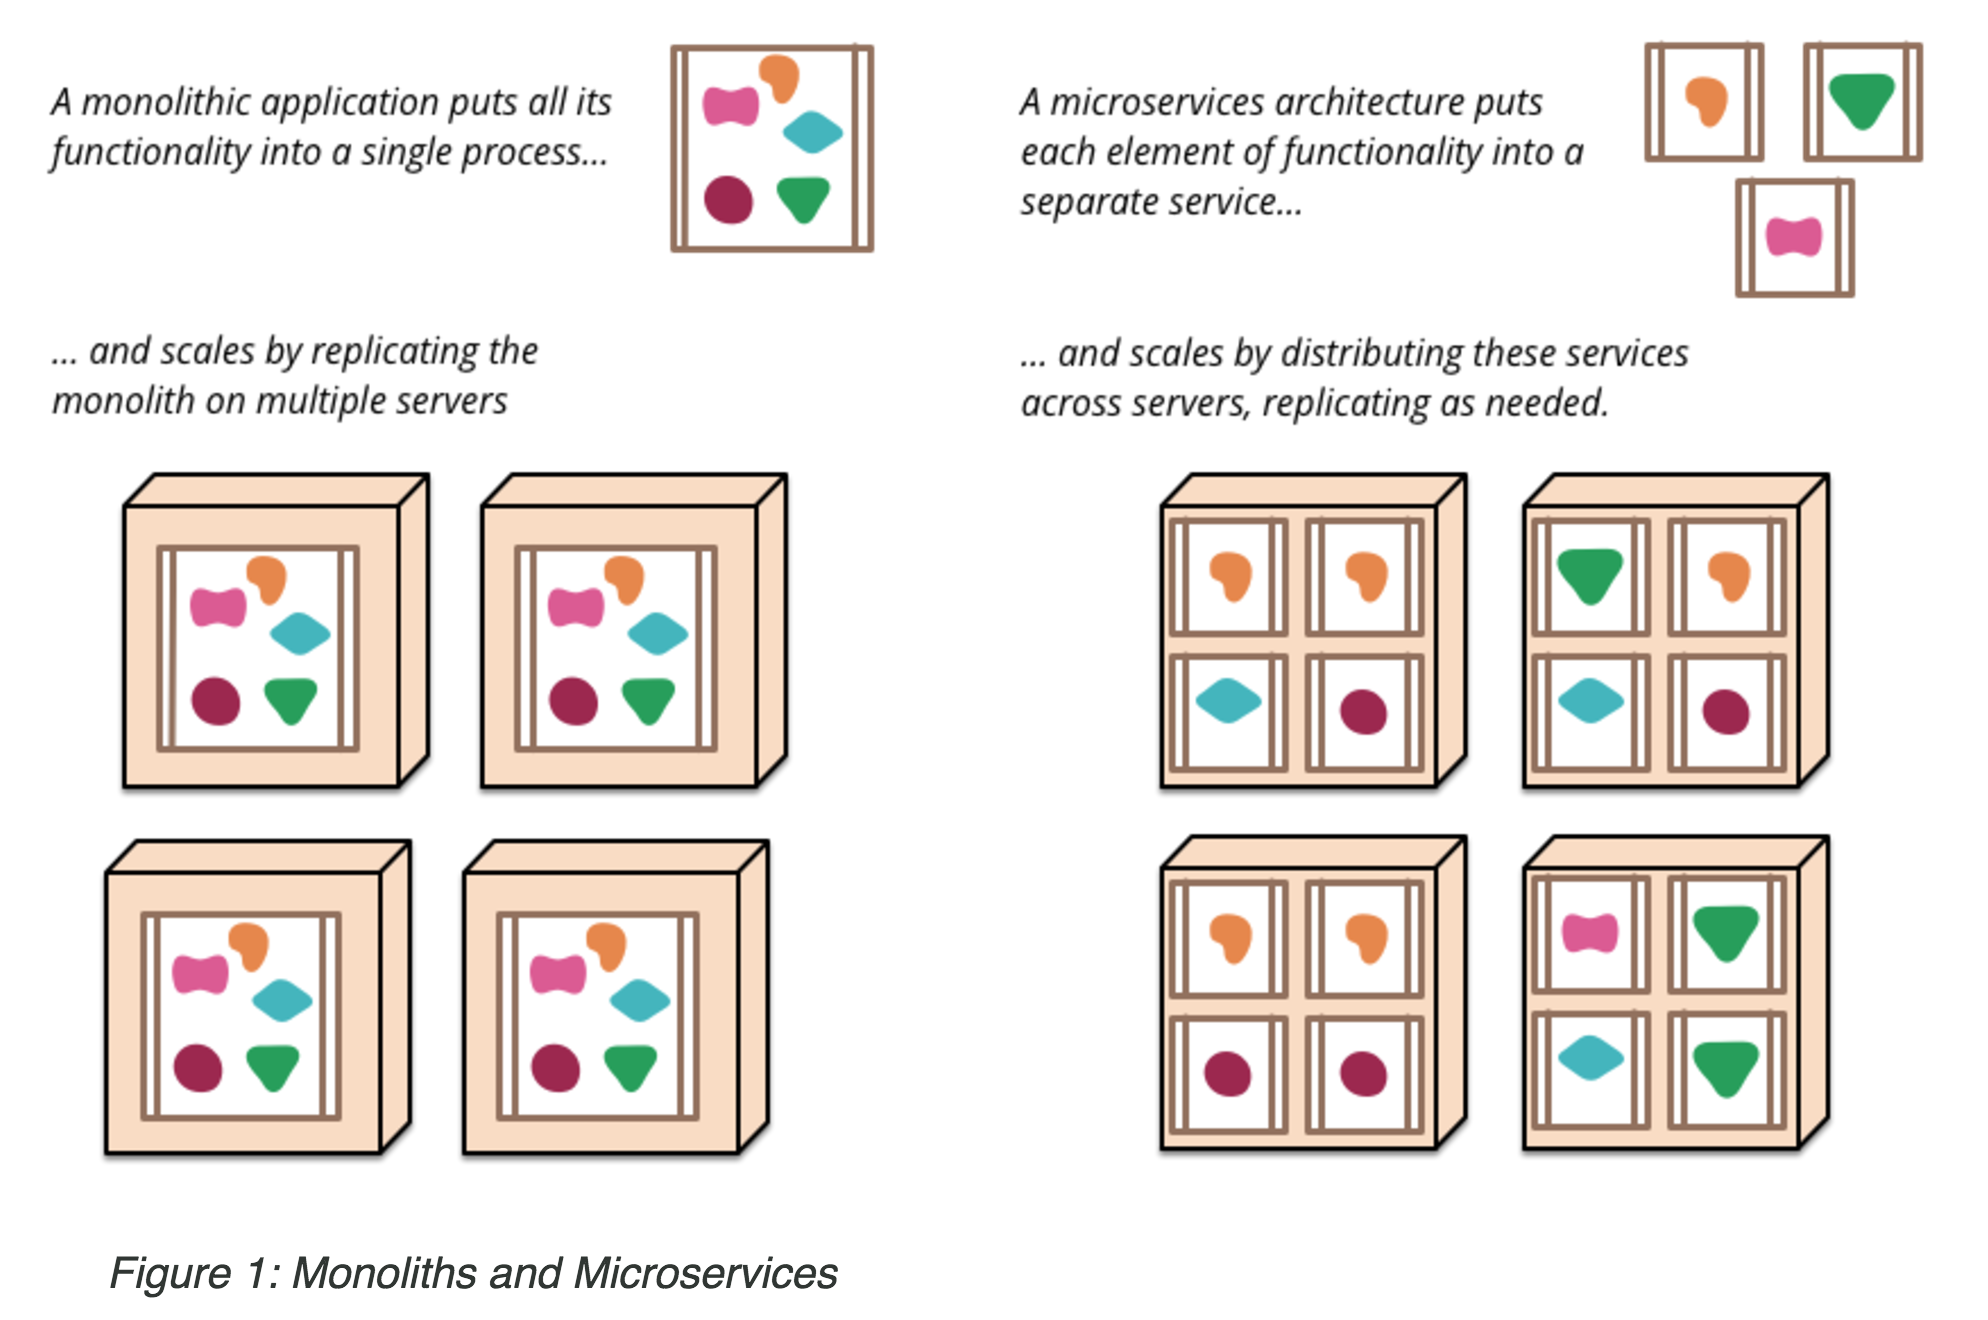
\includegraphics[scale=0.12]{architecture_microservice_definition}  
  \caption{A microservice architecture, consisting of individual executable in their own run-time environment. Each environment is replicated to satisfy load. A load balancer is put in front to distribute load.}
  \label{fig:architecture_microservice_definition}
  \end{center}
\end{figure}

At the same time microservices introduce more complexity. By having individual services, each service has it's own life cycle and can potentially fail. Microservices makes it necessary to have increased automation when deploying, monitoring and maintaining system health\cite{meshenberg2016microservices}.

According to Fowler the microservice architecture utilizes a subset of the original SOA term, it is therefore plausible to state that microservices not necessarily introduces anything new. At the same time a new term makes it possible to focus on specific and very usable parts of SOA. According to Fowler SOA is too broad a term, encapsulating too many aspects, making it too hard to reason about how SOA improves the working process when creating big distributed systems \cite[t.~13:22]{fowler2014microservicesoamonolith}.

As the microservice architecture was created out of a need for reducing complexity and improving agility and reliability \cite[p.~68]{long2017cloud} \cite[p.~192]{newman2015microservices}, different companies started developing microservice architectures independently. There is therefore no official definition of the architecture, but a set of defining characteristics, which are described in detail below.

\subsection{Defining characteristics}
There is a series of defining characteristics for services in a microservice architecture, which should be followed to avoid pitfalls when utilizing microservices. These characteristics describe what teams utilizing microservices often times do, there is no definitive definition of what a microservice architecture is.

\subsubsection*{Componentization via Services}
Componentization is used to decouple parts of an application, so that a service is only responsible for limited amount of highly related functionality\cite{morgantini2013whatAreMicroServices}. The componentization can initially be created by analysing the domain and identifying bounded contexts\cite[p.~31]{newman2015microservices}, each bounded context contains information only important internally in the context. 
The external important information is therefore made available through a interface, while internally important information is hidden from outsiders, simplifying boundaries.

By using services for componentization, a explicit interface is created, hindering tight coupling between components. Explicit remote call mechanisms are often used to facilitate communication between components. Communication through remote calls incur some resource and implementation overhead, being more resource intensive and harder to use than the traditional in process calls.

\subsubsection*{Splitting around Business Capabilities}
Services are organized around business capabilities, by analysing the domain carefully, each service can be limited in size and functional requirements. Each service implements all functionality to fulfil the identified requirements for that part of the business area, potentially consisting of multiple processes, developed and deployed together. A service could implement a application process having a underlying database exclusively used for that application process\cite{fowler2014microservices}.

\subsubsection*{Well Defined and Simple Communication Channels}
Keeping logic out of the communication method is important when developing microservices. Inspired by UNIX implementation, microservice architecture tries to delegate the entire concern of applying logic to the service implementations. When a service receives a request it applies its logic as appropriate and produces a response. The communication is often done with HTTP request-responses, defining the communication interfaces with a REST protocol\cite{fowler2014microservices}.

\subsubsection*{Decentralized Governance}
By decentralizing governance and organising around business capabilities, each service can be build and optimized to solve a very specific part of the domain \cite{fowler2014microservices}.
This is often paired with 'end-to-end' responsibility 
\note{Kunne potentielt tilføje hvordan team skills også kan splittes ud, samt hvordan det gør teams i stand til at sidde forskellige steder og arbejde med det samme}

\subsubsection*{Decentralized Data Management}
Services often have their own data store, decentralizing data management. Each service has the data that is relevant for that service, and not more. 

\note{Potentielt gør brug af Martin Fowler artikel "PolyglotPersistence", der snakker om brug af NoSQL teknologier}

\subsubsection*{Automation of Deployment}
Microservices infer a lot of operational complexity, as there are many services to deploy and monitor. The use of infrastructure automation techniques is necessary, improving insight into the quality of newly developed software, and reduce the time it takes to move new features from development to production\cite{newman2015microservices}. This is often achieved with build pipelines know from Continous delivery (CD), a build pipeline is seen on figure \ref{fig:architecture_microservice_build_pipeline}.

\begin{figure}[!htb]
  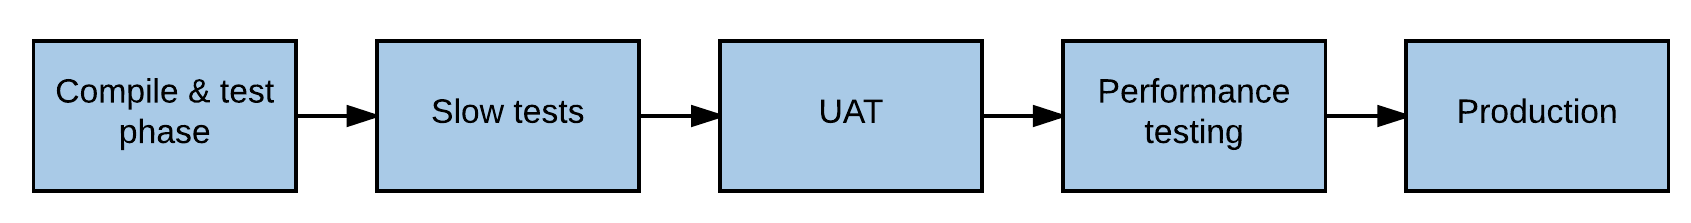
\includegraphics[scale=0.26]{architecture_microservice_build_pipeline}  
  \caption{Build pipeline(lend from Sam Newmann)}
  \label{fig:architecture_microservice_build_pipeline}
\end{figure}

\note {
\subsubsection*{Independently Deployable Services}
Each service is independently deployable, making it possible to add and update functionality in each service as needed.
}

\subsection{Derived qualities}
Microservices in it self presents a lot of benchmark benefits, giving possibility to control capacity, introduce redundancy and solve single point of failure issues, a microservice architecture improves overall application resilience if utilized correctly. At the same time microservices introduces additional complexity, because services has to communicate with dependent services using non-deterministic communication channels. This in turn has the effect of highlighting otherwise transparent challenges with integration points, causing engineers utilizing microservices to be more resilience aware, expecting failure between services. In a monolith implementation, a library dependency used in process might introduce new possible error states or undefined behaviour, but in this context software engineers tend to be less aware of the possible errors this dependency could incur. When having very clear interfaces with dependencies, engineers tend to take more precautionary measures. These measures are not directly measurable, but help create a more resilient system. 

\subsubsection*{Design for Failure}
A challenge with using services as components is the inherent complexity of communication over the wire, when two separate services need to communicate. In turn this highlights the existing pitfalls with every integration points, that exists even in a monolith architecture.

\subsubsection*{Sophisticated Real-Time Monitoring}
When designing many independent services, it is necessary to have sophisticated monitoring and logging, in order to control that services are running correctly. This enables engineers to know if any action needs to be taken to restore a fully functional system, or if service was automatically restored.

\note{
\section{Service discorvery}
C. Richardson, “Service discovery in a microservices architecture.” 
\url{https://www.nginx.com/blog/service-discovery-in-a-microservices-architecture/}


\section{Event-driven architecture}
\comment{This section is still in note form}
There are four patterns occurring in many of the systems where the word event-driven architecture.

Systems are often get very coupled because the different system depend on each other.


\section{Event notification}
It is a particular important part of the architecture. Subsystems communicate through events.

Applications subscribe to the events they are interested in, and react when an event comes along. 
By doing this you reverse dependencies.
Besides reversing dependencies, we now have a record that can be referred to and passed around, when an event happens. 'Bottling it op'.

What is the difference between events and commands. Events does not expect any specific reaction, but are just informing about change. Commands imply certain reaction to a event.

It allows us to hook up many different system up to events, without incurring change in existing applications. It easily allows to implement new features, without changing other

At the same time it removes easy observable flow. There is no code to look at, you have to debug.

\subsection{Event-carried State Transfer}
Downstream services duplicate the data they receive from events, removing the need for calls to the emitter. Less traffic is required, because more information is put into the events. Subscribing services can therefore deduct what to do from events, without contacting the emitter for additional data. The event therefore contains all the data that downstream systems want to have.

Downstream services therefore need to store the events they are interested in. 

It reduces the calls to the emitter, reducing traffic. Can improve availability, consumers are not directly tied to the emitter, the consumer has it's own data and can therefore continue operation if the emitter goes down.

This introduces lack of consistency. This is a less common pattern, but it can be a good one to utilize in some cases.

\subsection{Event Sourcing}
Changes are registered, by putting event on top of a event stack or log, the event is thereafter processed, updating the application state.

The Log can rebuild application state at any time.

In case of changes:
1. Event object is created - 'Address change' - pop into a seperate storage area
2. Process event - 'Change address'

Event sourcing works on customer state the way subversion works on code.

It is often a combination of all events and some 'snapshots'. Snapshots are sometimes done, 'closing out the year' ignoring events that has happened earlier, simplify the events, making it easier to reason about future events. Storage is therefore a mixture of events and snapshots. But you always want to be able to reason about the current state.

This pattern have several benefits:
Audit
Debugging, realy usefull to be able to go back and forth in state.
Historic state, if a error has occurred in the past, the difference it would make in current state can be calculated by going back and changing an event and calculating the difference.
Alternative state, you have a alternative to storing application state, by storing it in live memory. You still have to have an alternative store, so you can recreate state.

Disadvantages:
Unfamiliar, harder to work with
External system, gets a bit more complex, cannot ask the system for events again. Therefore a replay mechanism has to be made, to be able to restore application state. Has to save events.
Event Schema, how are events stored, so they can be replayed while the application that processes them is changed around them.
Identifiers, Traps when trying to make it possible to replay application state.
Potential disadvantages:
Asynchrony, adds complexity as it is introduced to handle emitting and handling events. It does not have to be used though.
Version, It can be hard to reason about. If application state structure is changed, can the application the still process year old events. Snapshots can be cut down two one day, so this is not a problem.

Pros and cons. Advantages and disadvantages.

\subsection{Command Query Responsibility Segregation}
Seperate pieces of software components that read and write to the central store.

Command model, write the model. It is only used when making updates.

Query model, 

It is appropriate pattern, but seems to 
}